\documentclass[letterpaper, 11 pt]{article}
\usepackage{amsmath}
\usepackage{siunitx}
\usepackage{natbib}

%Image pkgs
\usepackage{float}
\usepackage{graphicx}
\graphicspath{ {images/} }
\usepackage{subcaption}

%Algorithm display pkgs
\usepackage{algorithm} 
\usepackage{algpseudocode}

%Content formatting
\addtolength{\oddsidemargin}{-.875in}
\addtolength{\evensidemargin}{-.875in}
\addtolength{\textwidth}{1.75in}

\addtolength{\topmargin}{-.875in}
\addtolength{\textheight}{1.75in}

\title{\Large \bf Auger-driven Motion in Granular Media}
\author{\centering Stephanie L. Chang and Paul B. Umbanhowar}

\begin{document}
\pagenumbering{arabic}
\maketitle

\begin{abstract}
Brief summary of project and results
\end{abstract}

\tableofcontents

\section{Introduction}

Why this project is interesting and important for the industry today
Goal underground locomotor follow arbitrary trajectories
Many geometries tried Maladen, push me pull me, etc. 

\section{Approach}
Description on how I intended to build and test a robot in poppy seeds and created a mathematical model based off of Francisco's recent paper to optimize the parameters.  
Wings to counteract torque.

Initial idea to make and try.

Describe why we built it as it was and why we decided not to go with certain designs like the double screw. Modular for easy assembly and localized testing. 

\section{Iteration Progression}

\section{Analytical Optimization}
More informed view of what we are doing. 
Describe what Francisco's model claims in depth and how we expanded on it to describe helical motion for augers. 
Talk about the idea of using Chen's friction coefficients to account for the variability of forces on auger in relation to the angle of the sweep.  
force bal to find propulsive force

\begin{algorithm}[H]
	\caption{Auger Local Inclination Optimization}
	\label{augerOpt}
	
	\begin{algorithmic} %Program set-up
	\State \textbf{Knowns:}
	\State $R, n, d, \omega$ \Comment Auger radius, number of turns, auger depth, and angular velocity
	\State $0<\varepsilon \ll 1$
	\State $F_x(\phi,U)$ \Comment Thrust in the horizontal direction
	\State
	\State \textbf{Compute:} Maximum helix translational speed $U$ for different $\phi$ values
	\end{algorithmic}
	
	\begin{algorithmic}[1] %Program process
	\State Calculate $C_n$ and $C_t$ \Comment Normal and tangential friction coefficients 
	\State Let $\phi = 10*\frac{\pi}{180}$
	\While{$\phi < 90*\frac{\pi}{180}$}
		\State $U_{guess} = \varepsilon$ \Comment Initialize helix x-direction speed close to 0 
		\While{$F_x(\phi, U_{guess}) > \varepsilon$} \Comment Modified Newton-Raphson*
			\State $U_{guess} = U_{guess} - \frac{F_x(\phi, U_{guess})}{\frac{d}{dU}F_x(\phi,U_{guess})}$
		\EndWhile
		\State Store $\phi$ and $U_{guess}$ 
		\State $\phi = \phi + (1*\frac{\pi}{180})$ \Comment Increment $\phi$ by 1 degree
	\EndWhile
	\State Find the $\phi$ which corresponds to the largest $U_{guess}$ saved
	\end{algorithmic}
\end{algorithm}
*Omitting the absolute value operator ensures that Newton-Raphson will not be employed to solve for the $U$-intercept when the line tangent at $U_{guess}$ crosses the $U$-axis at a value $\leq 0$. This is necessary because function $F_x(\phi,U)$ contains natural log terms.       
 
\medskip
To verify the theoretical model proposed in \cite{Melo}, an equation for $F_x(\phi,U)$ was derived using the resistive-force theory. An illustration of the cylindrical coordinate system ($\vec{e_r}, \vec{e_\theta}, \vec{e_x}$) used to describe the helix can be seen in Figure~\ref{fig:helix_csys}. Local inclination angle $\phi$, shown in Figure~\ref{fig:helix_phi}, was used to define tangential unit vector $\vec{e_t} = \left\langle 0, \cos(\phi),\sin(\phi)\right\rangle $ and normal unit vector $\vec{e_n} = \left\langle 0, \sin(\phi), -\cos(\phi)\right\rangle $. The local velocity of a wire segment with respect to the helix base was also confirmed to be $\vec{\nu} = \left\langle 0, rw, U\right\rangle $.

\begin{figure}[H]
\centering
\begin{subfigure}{.5\textwidth}
	\centering
	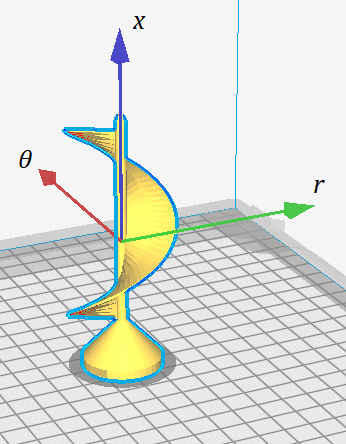
\includegraphics[height=6cm]{./helix_csys}
	\caption[Helix coordinate system]{Helix coordinate system}
	\label{fig:helix_csys}
\end{subfigure}%
\begin{subfigure}{.5\textwidth}
\centering
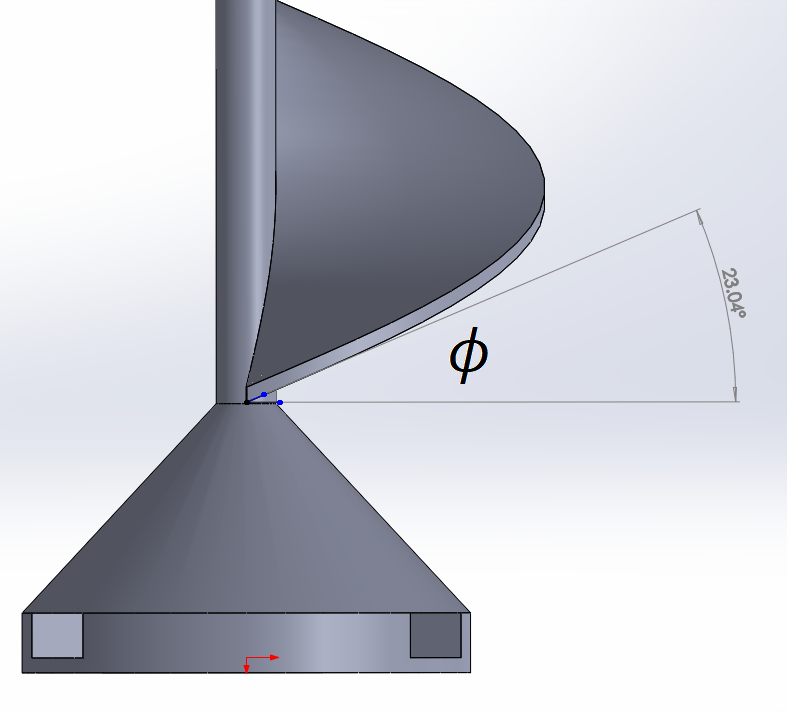
\includegraphics[height=6cm]{./helix_phi}
\caption{Local inclination angle $\phi$}
\label{fig:helix_phi}
\end{subfigure}
\caption{Problem set-up}
\label{probSetup}
\end{figure}

For a thin coil ($R_{wire} \ll R_{helix}$), the net force per unit length felt by a small section along the helix path was found to be 
\begin{equation}\label{f}
\begin{split} 
\vec{f} &= -C_t(\vec{e_\nu}\cdot\vec{e_t})\vec{e_t}-C_n(\vec{e_\nu}\cdot\vec{e_n})\vec{e_n} \\
&=\frac{-C_t(rw\cos(\phi)+U\sin(\phi))\vec{e_t}-C_n(rw\sin(\phi)-U\cos(\phi))\vec{e_n}}{\sqrt{U^2+(rw)^2}}\ \text{.}
\end{split} 
\end{equation}
Integrating over the full length of the coil, the total amount of propulsive force generated by the screw in the x-direction was discovered to be  
\begin{equation}\label{FxCoil}
\begin{split}
F_x &= \int_{0}^{2 \pi n}(\vec{f}\cdot\vec{e_x})\frac{r}{\cos(\phi)}d\theta \\
&=\frac{2\pi nr}{\cos(\phi)}\frac{(C_n-C_t)r\omega\sin(\phi)\cos(\phi)-U(C_t\sin^2(\phi)+C_n\cos^2(\phi))}{\sqrt{U^2+(rw)^2}}\ \text{,}
\end{split}
\end{equation}
where $\vec{e_x} = \left\langle 0,0,1 \right\rangle $. For a particular case mentioned in \cite{Melo}, the approximate values of $C_t$ and $C_n$ were determined using 
\begin{equation}
\frac{C_n}{C_t} = \frac{1+\tilde{U}_m}{1-\tilde{U}_m/\tan(\phi)}\ \text{,}
\end{equation}
where $\tilde{U}$ = \SI[per-mode=fraction]{0.11}{\m\per\s} and $\phi$ = \SI{16}{\degree}, and 
\begin{equation}
C_n - C_t = cd\rho gh
\end{equation} 
where $c$ = 24, $d$ = \SI{0.003}{\m}, effective granular material density $\rho$ = \SI[per-mode=fraction]{1.45e3}{\kg\per\m^3}, $g$ = \SI[per-mode=fraction]{9.81}{\m\per\s^2} and $h$ = \SI{0.05}{\m}.

Plugging equation (\ref{FxCoil}), $C_t$, and $C_n$ into algorithm 1, Figure~\ref{MeloUvsPhi} was obtained. Although $C_t$ and $C_n$ depend on    

Give expressions for Chen's Ct and Cn. 


\section{Results}
Describe what was seen with the first blind test. Problems encountered. 
How the following iterations were changed to compensate. 
Wider screw, modular wings, captured nuts for easier assembly and better interfacing with adapter, brass adapter for motor shaft to counter wt imbalance and keep the screw on since the PLA kept wearing after a while. 

Describe results with math model. 
Replication of Francisco's wire model with constant experimentally derived Ct and Cn values
Implementation of Francisco's model with Chen's coeff
Our full Fx model with...whatever coeff end up being proper

limitations with printer

\section{Analysis}
Speculate all the things as to why things failed or not?

\section{Future Direction}
Future direction

\bibliographystyle{plain}
\bibliography{burrowing_biblio}

\end{document}